\documentclass{article}
\usepackage[utf8]{inputenc}
\usepackage{graphicx}
\usepackage{geometry}
\geometry{a4paper, total={16cm, 24cm}, top=2cm}
\usepackage{amsmath}
\usepackage{blindtext}
\graphicspath{ {img/} }
\usepackage{listings}
\usepackage{color}
\usepackage{hyperref}
\hypersetup{
    colorlinks=true,
    linkcolor=blue,
    filecolor=magenta,      
    urlcolor=cyan,
    }
\definecolor{dkgreen}{rgb}{0,0.6,0}
\definecolor{gray}{rgb}{0.5,0.5,0.5}
\definecolor{mauve}{rgb}{0.58,0,0.82}

\lstset{ frame=tb,
  language=C,
  aboveskip=3mm,
  belowskip=3mm,
  showstringspaces=false,
  columns=flexible,
  numbers=left,
  basicstyle={\small\ttfamily},
  numberstyle=\tiny\color{gray},
  keywordstyle=\color{blue},
  commentstyle=\color{dkgreen},
  stringstyle=\color{mauve},
  breaklines=true,
  breakatwhitespace=true,
  tabsize=3  
}


\title{Week 5 Programming Assignment}
\author{Steffen Petersen | au722120}
\date{October 3rd 2022}

\begin{document}
%\tableofcontents


\maketitle
\section{}
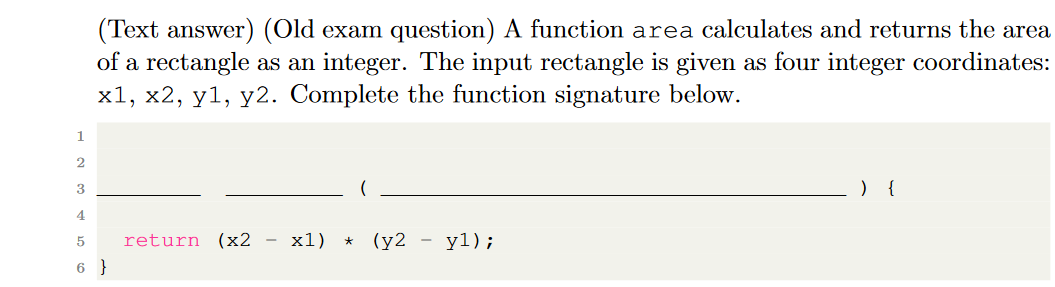
\includegraphics[width=\linewidth, keepaspectratio=true]{task1}
\vspace{2pt}\\
Below is my completed function, the same can be found in the task1.c file in the attached "Week 4 code.zip" folder, which includes a main function to test the get\_min function.
\begin{lstlisting}
  int get_min(int list[], int n) // A function that returns the lowest value in the given array list[] of length n.
  {
    assert(n > 0); // Precondition: Can't have an array with the length of 0 or lower.
    int lowest = list[0]; // Initialize the first "lowest" value, as the first slot in the array.
    for(int i = 1; i < n; i++){ // Run through the array from 0 -> n-1
      if(list[i] < lowest) // Test whether the current slot in the array has a lower value than the current saved lowest value.
        lowest = list[i]; // If above is true, lowest is reassigned as the value of the current spot in the array.
    }
    return lowest;
  } 
\end{lstlisting}


\section{}
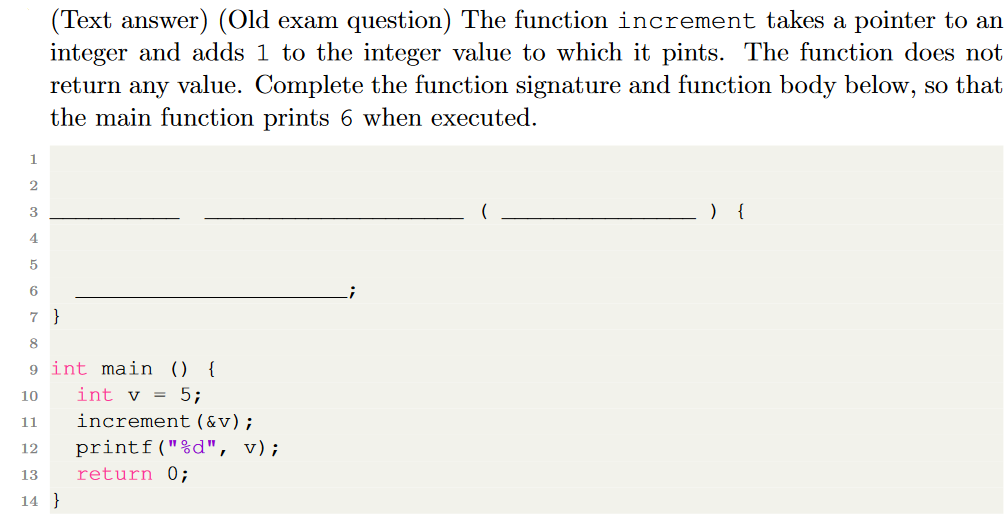
\includegraphics[width=\linewidth, keepaspectratio=true]{task2}
\vspace{2pt}\\
Below is my completed function, the same can be found in the task2.c file in the attached "Week 4 code.zip" folder, which includes a main function to test the reverse function.
\begin{lstlisting}
  void reverse(int list[], int rev_array[], int n) // A function to print an array in reverse order through a new array holding the values in reverse.
  {
    assert(n > 0); // Precondition: Can't have an array with the length of 0 or lower.
    for(int i = 0; i < n; i++){ // Run through the array from 0 -> n-1
      rev_array[i] = list[n-i-1]; // Assign the reverse array's value i, as the "opposite" value of list. So, rev_array's starting value becomes list's end value.
    }
    printf("The reverse of the function is as follows\n");
    for(int i = 0; i < n; i++) { // Print the reversed array
      printf("Slot %d : %d\n", i, rev_array[i]);
    }
  }
\end{lstlisting}




\section{}
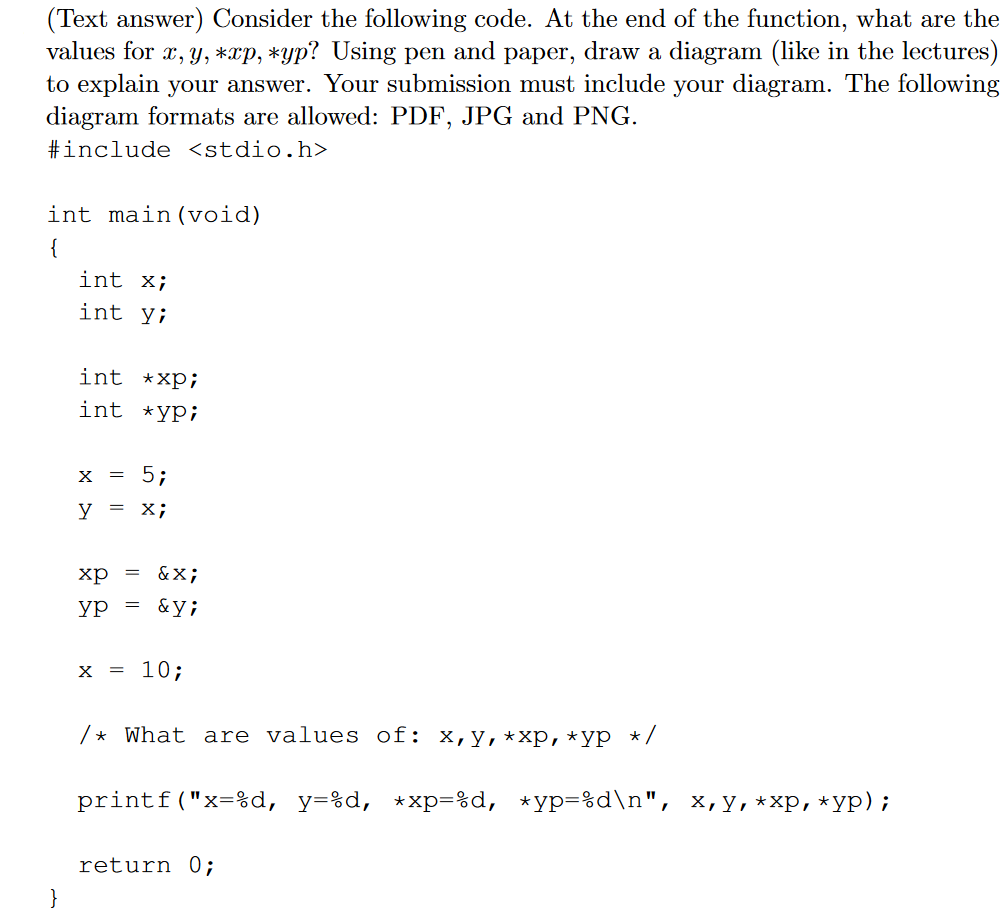
\includegraphics[width=\linewidth, keepaspectratio=true]{task3}
\vspace{2pt}\\
Below is my completed function, the same can be found in the task3.c file in the attached "Week 4 code.zip" folder, which includes a main function to test the longest\_seq function.
\begin{lstlisting}
  int longest_seq(int list[], int n) 
  {
      assert(n > 0); // precondition, size has to be greater than 0.
      int counter = 0; // Counter for current sequence of zeros
      int countmax = 0; // Record what our longest sequence has been so far.
      int index = -1; // Start index for position of zeros sequence at -1 (as the assignment shows.)
      
      for(int i = 0; i < n; i++){
          if(list[i] == 0){ // Check if current value of array is 0, if so, count 1 up
              counter++;
          }
          else counter = 0; // reset counter if we no longer are getting a sequence of 0's.
          if(counter > countmax){ // If current counter exceeds previous max, update the index to match where we started counting this sequence.
              index = i+1-counter; 
              countmax = counter; // Also update countmax.
          } 
      }
  return index;
  }
\end{lstlisting}

\section{}
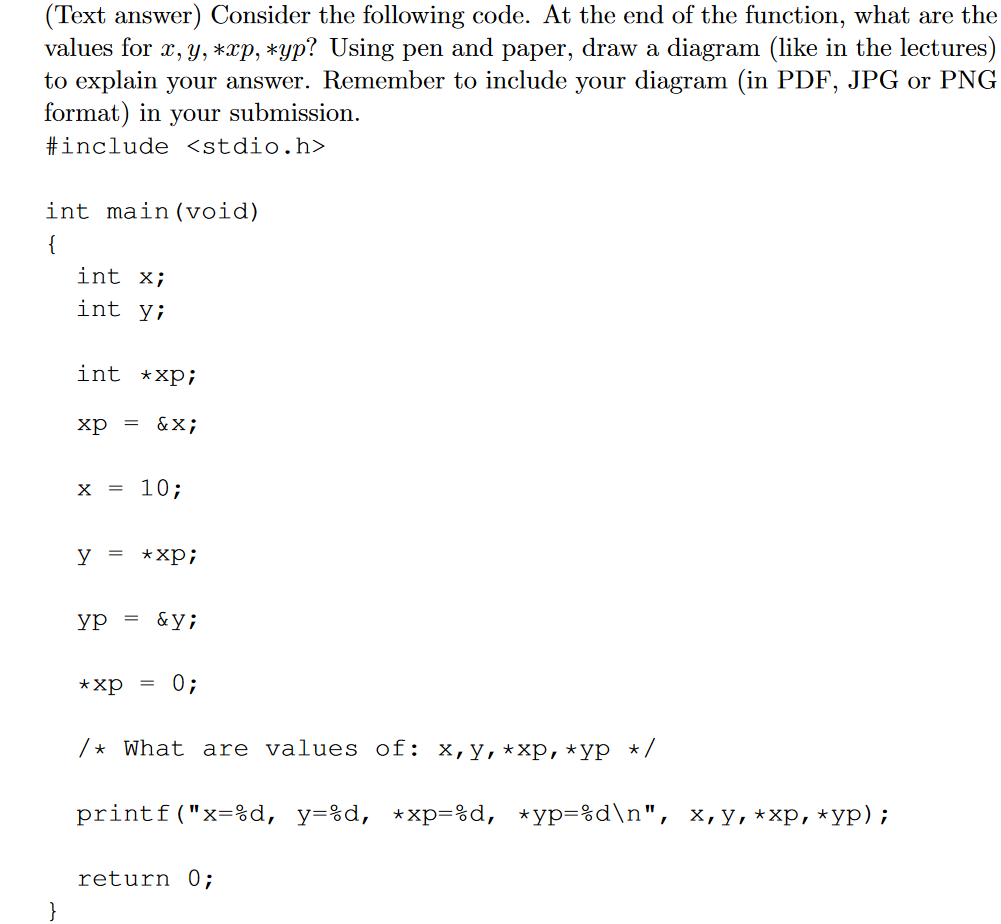
\includegraphics[width=\linewidth, keepaspectratio=true]{task4}
\vspace{2pt}\\
Below is my completed function, the same can be found in the task4.c file in the attached "Week 4 code.zip" folder, which includes a main function to test the count\_1\_to\_20 function.
\begin{lstlisting}
  void count_1_to_20(int a[100][150], int count[20]) 
  {	
    for(int rst = 0; rst < 20; rst++){
      count[rst] = 0; // Make sure the counter array is reset to 0.
    }
    // Precondition a only contains numbers from 1 to 20. (The programs runs fine regardless)
    for(int i = 0; i < 100; i++){ // Run through the first parameters 100 values
      for(int i2 = 0; i2 < 150; i2++){ // Run through the 2nd parameters 150 values, for each of the 100 outer values.
        count[a[i][i2]-1]++; //Counts +1 for each value from 1->20 in the entirity of a.
      }
    }
    for(int i3 = 0; i3 < 20; i3++){ // Output the results.
      printf("Nr. of %d's in the input: %d\n", i3+1, count[i3]); 
    }
  }
\end{lstlisting}
\pagebreak

\section{}
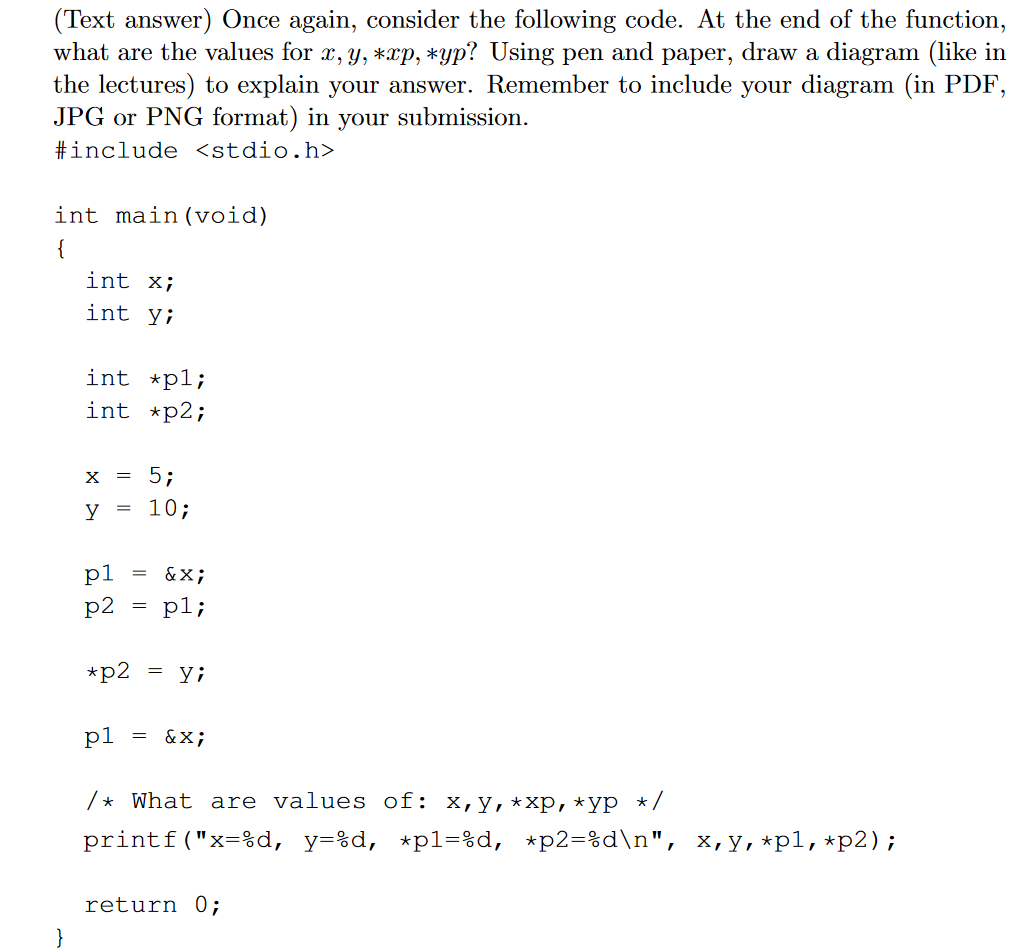
\includegraphics[width=\linewidth, keepaspectratio=true]{task5}
\vspace{2pt}\\
For this function I've used the return type double instead of void, as we would like to return the average value of the contents of the array, which double seems suitable for.\\
Below is my completed function, the same can be found in the task5.c file in the attached "Week 4 code.zip" folder, which includes a main function to test the average function.
\begin{lstlisting}
  double average(double list[], int n) // return type double to retain the best possible accuracy.
  {	
      double average; // Variable to store the ongoing sum and at last the average.
      for(int i = 0; i < n; i++){ 
          average += list[i];
      }
      average /= n; // Divide the sum of the whole array's values by its length, to get the average.
      return average;
  }
\end{lstlisting}


\section{}
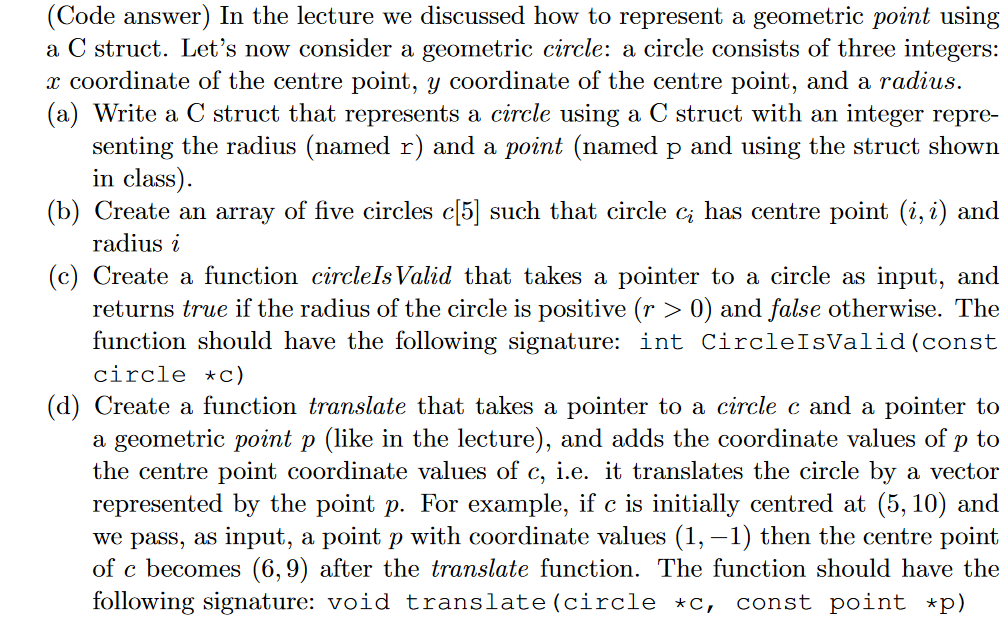
\includegraphics[width=\linewidth, keepaspectratio=true]{task6}
\vspace{2pt}\\



\section{}
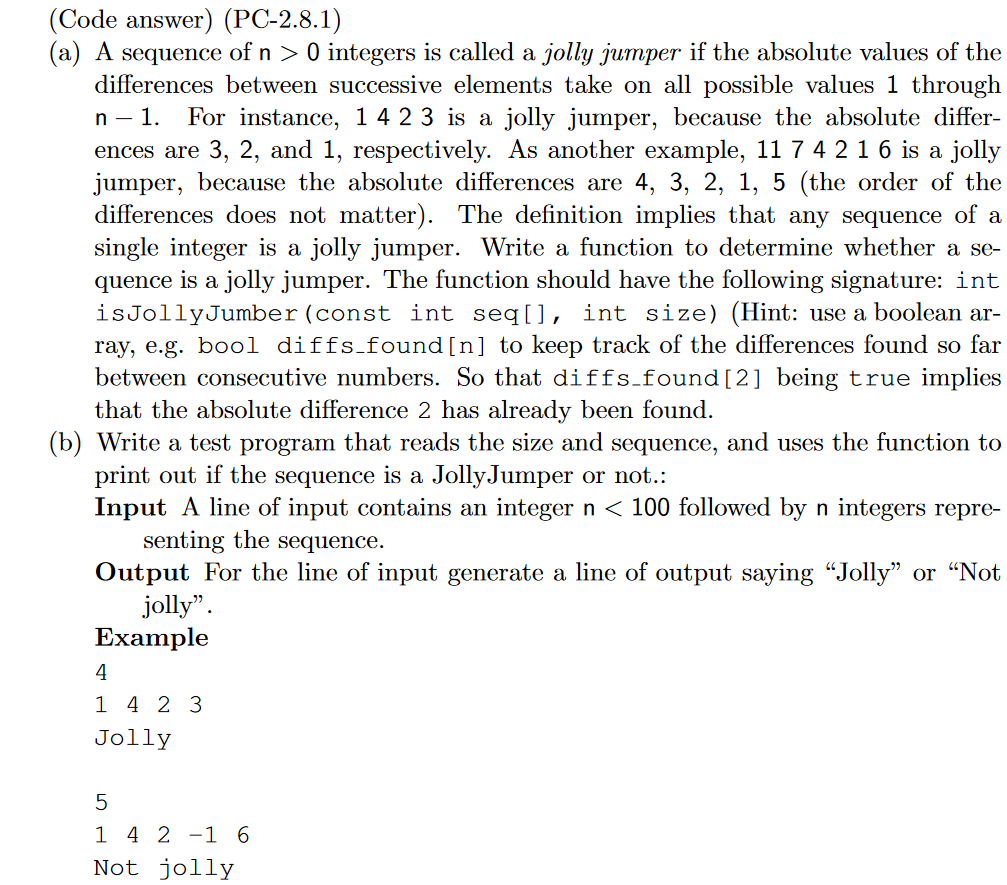
\includegraphics[width=\linewidth, keepaspectratio=true]{task7}
\vspace{2pt}\\


\end{document}